\documentclass[11pt,a4paper]{scrreprt}
\usepackage[utf8]{inputenc}
\usepackage[english]{babel}
\usepackage[margin=2.4cm]{geometry}
\usepackage{graphicx}
\usepackage{float}
\usepackage{array}
\usepackage{longtable}
\usepackage{booktabs}
\usepackage{tabularx}
\usepackage{enumitem}
\usepackage[table]{xcolor}
\usepackage{microtype}
\usepackage{underscore}
\usepackage[bookmarks=true]{hyperref}

\hypersetup{
    pdftitle={Software Requirements Specification -- CampusXchange},
    pdfauthor={Garav Goyal, Dhruv Rajput, Parth Zutshi, Harjap Singh Benipal},
    pdfsubject={UCS503P Software Engineering Laboratory},
    colorlinks=true,
    linkcolor=blue!60!black,
    citecolor=black,
    urlcolor=purple,
    linktoc=page
}

\def\myversion{1.0}
\setlist{itemsep=2pt,topsep=4pt}
\renewcommand{\arraystretch}{1.25}
\newcolumntype{L}[1]{>{\raggedright\arraybackslash}p{#1}}

% Functional-requirement table: ID | Requirement | Priority | Status
\newenvironment{reqtable}{%
  \small
  \begin{longtable}{>{\raggedright\arraybackslash\ttfamily\footnotesize}p{2.05cm} L{8.85cm} L{1.45cm} L{2.05cm}}
  \toprule
  \normalfont\normalsize\textbf{ID} & \textbf{Requirement} & \textbf{Priority} & \textbf{Status}\\
  \midrule\endhead
  \bottomrule\endfoot
}{\end{longtable}}

\newcommand{\impl}{Implemented}
\newcommand{\partl}{Partial}
\newcommand{\planned}{Planned}

\begin{document}

% ================= TITLE PAGE =================
\begin{titlepage}
\begin{flushright}
    \rule{16cm}{5pt}\vskip1cm
    \begin{bfseries}
        \Huge{SOFTWARE REQUIREMENTS\\ SPECIFICATION}\\
        \vspace{1.2cm}
        for\\
        \vspace{1.2cm}
        CampusXchange\\[0.3cm]
        \Large{A Campus-Verified Marketplace for Selling, Lending and Exchange}\\
        \vspace{1.2cm}
        \LARGE{Version \myversion}\\
        \vspace{1.2cm}
        \large
        Prepared by (Group 3C-14, BE Third Year, CSE):\\[0.2cm]
        1. Garav Goyal (1024030098)\\
        2. Dhruv Rajput (1024030102)\\
        3. Parth Zutshi (1024030116)\\
        4. Harjap Singh Benipal (1024030118)\\
        \vspace{1.2cm}
        Submitted to: Dr. Anushka\\
        UCS503P -- Software Engineering Laboratory\\
        \vspace{1.2cm}
        Computer Science and Engineering Department\\
        Thapar Institute of Engineering and Technology, Patiala\\
        \vspace{0.8cm}
        October 2026\\
    \end{bfseries}
\end{flushright}
\end{titlepage}

\tableofcontents

% =====================================================================
\chapter{Introduction}

\section{Purpose}
This Software Requirements Specification (SRS) describes the functional and
non-functional requirements of \textbf{CampusXchange}, a mobile marketplace
in which verified students of Thapar Institute of Engineering and Technology
can sell, lend and exchange everyday items such as textbooks, calculators,
lab gear, cycles and electronics.

The document is the agreed reference for what the system must do. It is
written to be consistent with the project proposal approved on
19 August 2026, and it records explicitly where the design has since been
refined (Section~\ref{sec:deviations}). It covers the complete system,
including the payment, handoff and dispute modules that are designed but
not yet implemented at the time of writing.

\section{Document Conventions}
\begin{itemize}
  \item Every requirement carries a unique identifier: \texttt{FR-<area>-<n>}
    for functional requirements, \texttt{NFR-<area>-<n>} for non-functional
    requirements and \texttt{BR-<n>} for business rules.
  \item \textbf{Priority} is one of \emph{High} (essential to the core
    workflow; the system is not usable without it), \emph{Medium}
    (important, but the core workflow still functions without it) or
    \emph{Low} (desirable enhancement).
  \item \textbf{Status} records progress at the time of writing:
    \emph{Implemented} (built and verified on device), \emph{Partial}
    (built, but part of the requirement is not yet enforced) or
    \emph{Planned} (fully designed and modelled; database support exists;
    implementation scheduled for the next phase).
  \item The words \emph{shall} (mandatory), \emph{should} (recommended)
    and \emph{may} (optional) are used in their usual requirements sense.
  \item Database tables, columns and API routes appear in
    \texttt{monospace}.
\end{itemize}

\section{Intended Audience and Reading Suggestions}
\begin{itemize}
  \item \textbf{Course instructor and evaluators} -- Chapter~1 and 2 for scope
    and context; Chapter~3 and 5 for the requirements themselves.
  \item \textbf{Developers (the project team)} -- Chapters~3, 4 and 6 give the
    exact behaviour, interfaces and data model to build against.
  \item \textbf{Testers} -- every requirement in Chapters~3 and 5 is written
    to be verifiable; Chapter~8 lists the acceptance criteria.
  \item \textbf{Pilot administrators / moderators} -- Sections~3.4, 3.9 and
    3.11 describe their responsibilities in the system.
\end{itemize}

\section{Product Scope}
Campus commerce today runs on hostel WhatsApp groups, batch chats and
noticeboards that were never designed for hundreds of people who mostly do
not know each other to trade safely. CampusXchange replaces these with a
single, college-only app in which:
\begin{itemize}
  \item only holders of a valid \texttt{@thapar.edu} address can register,
    and each account also carries a roll number and an administrator-reviewed
    student ID card;
  \item items can be listed for \textbf{Sell}, \textbf{Lend/Rent} or
    \textbf{Exchange (barter)} from one unified, searchable feed;
  \item no listing is published until an administrator has reviewed it;
  \item buyers and sellers negotiate through in-app chat and structured
    offers that the system records;
  \item payment is held in escrow and released only after a QR-verified,
    in-person handoff on campus, with condition photographs as evidence;
  \item disputes are adjudicated by an administrator using that evidence.
\end{itemize}

\textbf{Out of scope} for this version: shipping or courier delivery,
cross-campus listings, a custom-trained machine-learning model, OCR or
third-party KYC verification of ID documents, and a separate web
application for students.

\section{Project Objectives}
\begin{enumerate}[label=\textbf{O\arabic*.}]
  \item \textbf{Verified access:} restrict participation to genuine Thapar
    students, enforced in the database rather than only in the client.
  \item \textbf{Unified listing surface:} one searchable, filterable feed
    covering Sell, Lend and Exchange.
  \item \textbf{Moderated publication:} no listing reaches the public feed
    without passing through human review.
  \item \textbf{Recorded negotiation:} price agreement is captured as
    structured offers rather than free-text chat.
  \item \textbf{Safe settlement:} escrow-held payment released only after a
    QR-verified handoff, with support for the lend return cycle.
  \item \textbf{Recourse:} an evidence-based dispute process run by
    administrators.
  \item \textbf{Measurable outcome:} median time-to-listing-clearance (TLC)
    of at most 4 hours during the pilot.
\end{enumerate}

\section{Definitions, Acronyms and Abbreviations}
\begin{longtable}{L{3.2cm} L{12cm}}
\toprule
\textbf{Term} & \textbf{Meaning}\\ \midrule\endhead
API & Application Programming Interface (here, the NestJS REST backend)\\
Admin & A user whose \texttt{users.role} is \texttt{admin}; performs moderation, ID verification and dispute resolution\\
Escrow & Holding a buyer's payment until the handoff is confirmed\\
Guest & A person using the app without signing in; may browse only\\
Handoff & The physical, on-campus meeting at which an item changes hands\\
Listing & An item offered for Sell, Lend or Exchange\\
OTP & One-Time Password, a 6-digit code sent to the student's college email\\
QR token & A signed, single-use, time-bound code that identifies one transaction at handoff\\
RLS & Row-Level Security (PostgreSQL feature)\\
Signed URL & A time-limited link to a private file in object storage\\
Student & A signed-up user whose ID card is not yet verified\\
Verified Student & A student whose \texttt{id_verified} is \texttt{verified}\\
TLC & Time to Listing Clearance: time from listing submission to moderation decision\\
UML & Unified Modeling Language\\
\bottomrule
\end{longtable}

\section{References}
\begin{enumerate}
  \item CampusXchange Project Proposal, UCS503P, submitted 19 August 2026.
  \item CampusXchange Mid-Semester Evaluation Report (\texttt{report/main.tex}).
  \item CampusXchange API Contract (\texttt{docs/api-contract.md}).
  \item CampusXchange database schema (\texttt{supabase/migrations/}).
  \item IEEE Std 830-1998, \emph{IEEE Recommended Practice for Software
    Requirements Specifications}.
\end{enumerate}

% =====================================================================
\chapter{Overall Description}

\section{Product Perspective}
CampusXchange is a new, self-contained product that replaces informal
group-chat trading. It follows a three-tier architecture
(Figure~\ref{fig:arch}):
\begin{itemize}
  \item \textbf{Mobile client} -- a React Native (Expo) app; the only
    user-facing surface. Students, guests and administrators all use it;
    administrators see an extra \emph{Review} tab.
  \item \textbf{Backend API} -- a stateless NestJS service organised into
    feature modules (profile, listings, chat, admin) behind a guard layer
    that authenticates every request.
  \item \textbf{Data platform} -- Supabase, providing PostgreSQL, the
    authentication service (email OTP) and object storage (a private
    \texttt{id-cards} bucket and a public \texttt{listing-images} bucket).
\end{itemize}
Authentication traffic goes directly from the app to the identity provider;
all application data passes through the backend.

\begin{figure}[H]
  \centering
  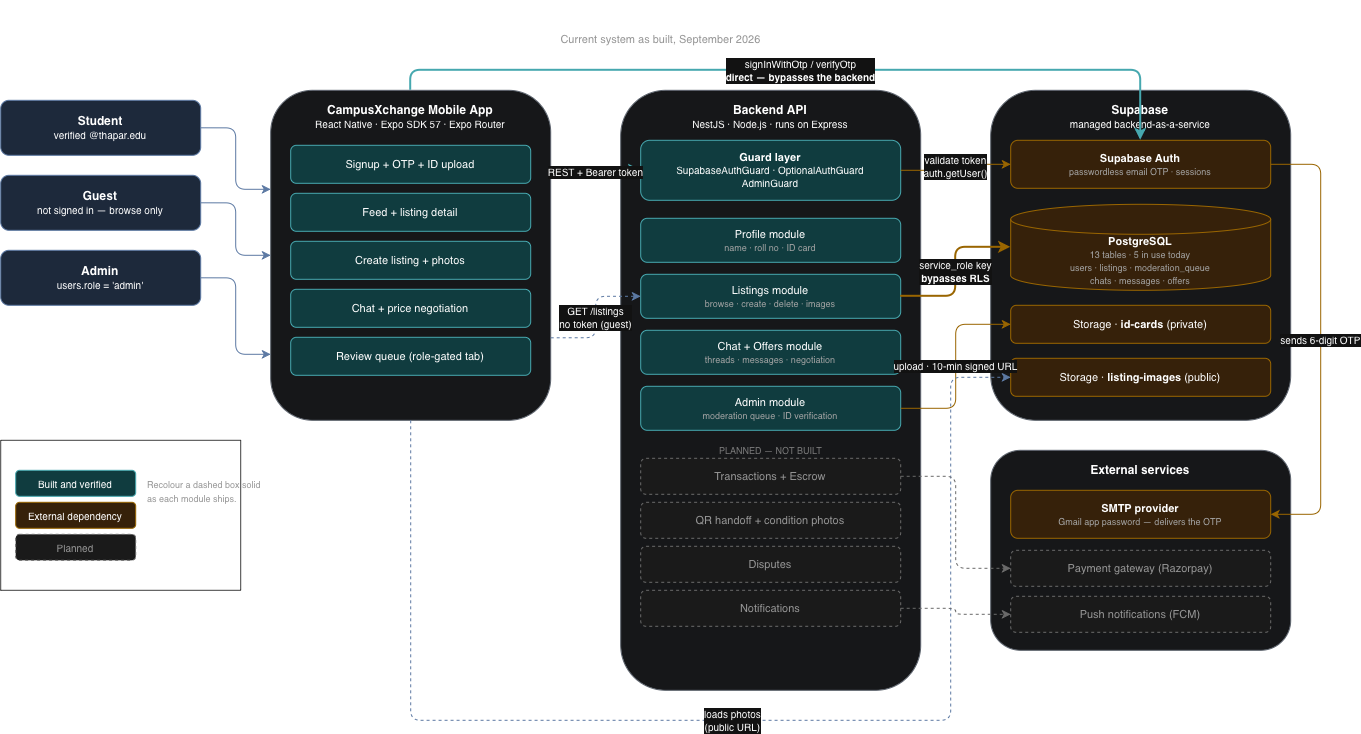
\includegraphics[width=\textwidth]{figures/architecture-highlevel.png}
  \caption{High-level system architecture (solid: implemented; dashed: planned)}
  \label{fig:arch}
\end{figure}

\section{Product Functions}
At a high level the system shall allow users to:
\begin{enumerate}
  \item sign up and log in with a college email and OTP, provide a roll
    number and upload a student ID card for verification;
  \item browse and search live listings by type and category, including as a
    guest;
  \item create, view and delete listings with photographs, condition and a
    campus meeting point;
  \item have every new listing reviewed by an administrator before it goes live;
  \item chat with the other party and negotiate a price through offers;
  \item pay into escrow, receive a QR code, and complete a verified handoff
    with condition photographs;
  \item complete a return leg for lend transactions;
  \item raise and resolve disputes;
  \item receive notifications and category-based alerts.
\end{enumerate}
Figure~\ref{fig:workflow} summarises the end-to-end workflow.

\begin{figure}[H]
  \centering
  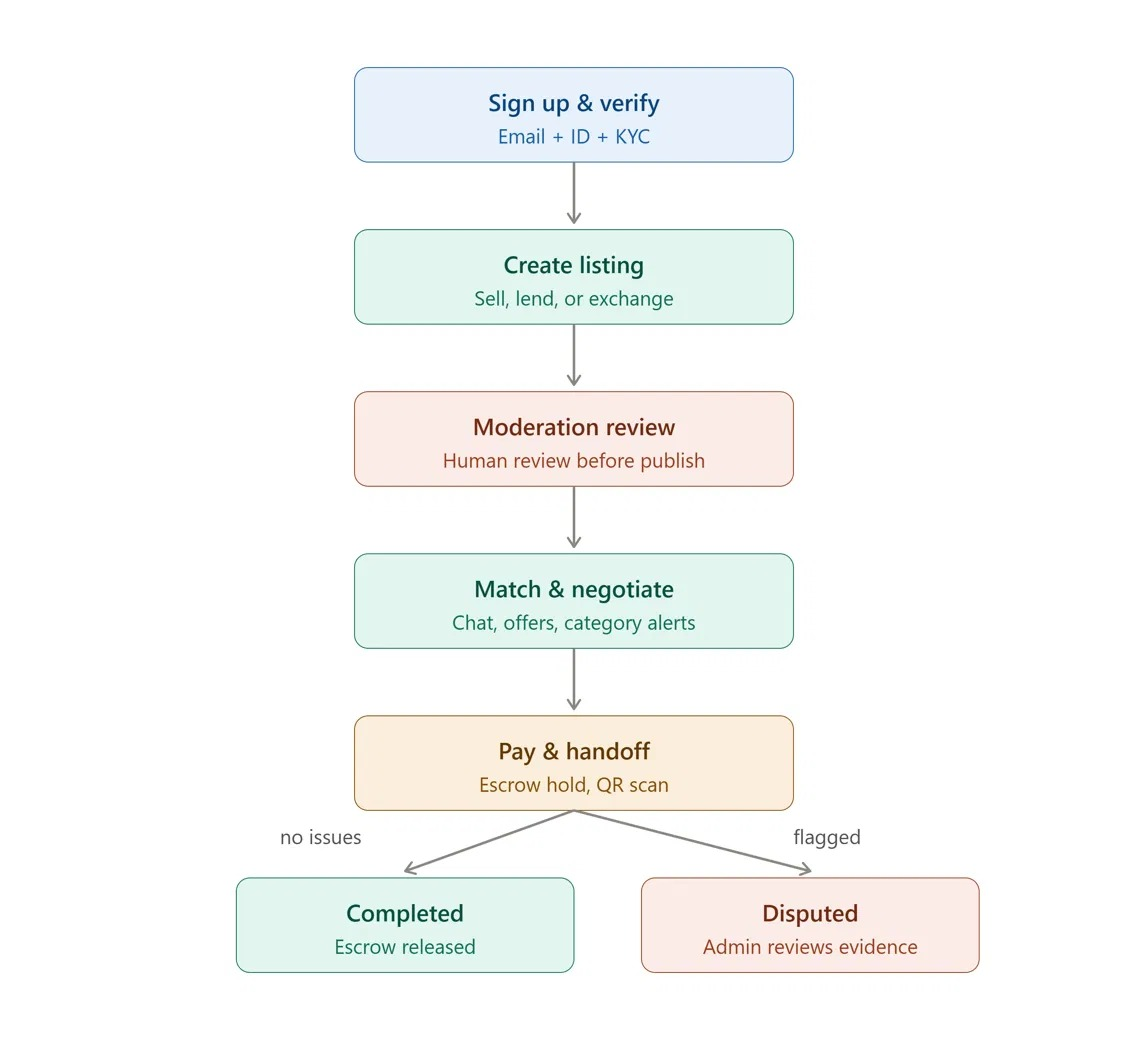
\includegraphics[width=0.62\textwidth]{figures/workflow-overview.jpg}
  \caption{End-to-end workflow of a CampusXchange transaction}
  \label{fig:workflow}
\end{figure}

\section{Stakeholders}
\begin{longtable}{L{3.6cm} L{11.6cm}}
\caption{Stakeholders and their interests}\label{tab:stakeholders}\\
\toprule
\textbf{Stakeholder} & \textbf{Interest in the system}\\ \midrule\endhead
Students (buyers, borrowers) & Find items cheaply and safely from people on their own campus\\
Students (sellers, lenders) & Reach the whole campus, get paid reliably, get borrowed items back\\
Administrators / moderators & Keep the marketplace free of unsafe or fake content; resolve disputes fairly with evidence\\
Thapar Institute & A safe, college-only trading space; protection of student identity data\\
Course instructor (Dr. Anushka) & A well-engineered, specified, tested and measurable project\\
Development team & Clear, realistic requirements to build and test against\\
External service providers & Supabase (auth, database, storage), payment gateway and push-notification service, whose limits constrain the design\\
\bottomrule
\end{longtable}

\section{User Classes and Characteristics}
\begin{longtable}{L{3cm} L{12.2cm}}
\caption{User classes}\label{tab:users}\\
\toprule
\textbf{User class} & \textbf{Description and permissions}\\ \midrule\endhead
Guest & Not signed in. May browse and search live listings and view listing details. The meeting location is hidden. Cannot chat, list, or transact.\\
Student & Signed in with a verified \texttt{@thapar.edu} email; ID card not yet approved. May browse, upload an ID card, set a roll number and receive alerts.\\
Verified Student & ID card approved by an admin. Inherits all Student rights and may additionally create listings, chat and negotiate, pay, complete handoffs and returns, and raise disputes.\\
Administrator & A student account with \texttt{role = admin}. Reviews ID cards, moderates listings, resolves disputes, applies penalties and views platform analytics.\\
Notification Service (external) & Secondary actor; delivers push/email notifications. Never initiates a use case.\\
Payment Gateway (external) & Secondary actor; collects payment and supports escrow hold, release and refund.\\
\bottomrule
\end{longtable}

Users are expected to be comfortable with smartphone apps, but may use
budget Android devices and unreliable hostel Wi-Fi. Administrators are
trained student volunteers or staff (2--3 in the pilot).

\section{Operating Environment}
\begin{itemize}
  \item \textbf{Client:} Android and iOS smartphones running the Expo
    (React Native, Expo SDK 57) app; during development, run through Expo Go.
  \item \textbf{Backend:} Node.js (v22) running NestJS; currently run
    locally, to be deployed on a cloud platform for the pilot.
  \item \textbf{Data platform:} Supabase-hosted PostgreSQL, Supabase Auth
    and Supabase Storage.
  \item \textbf{Network:} HTTPS over campus Wi-Fi or mobile data.
\end{itemize}

\section{Design and Implementation Constraints}
\begin{enumerate}[label=\textbf{C\arabic*.}]
  \item Sign-up is restricted to the \texttt{@thapar.edu} domain; single-campus
    pilot with no cross-campus visibility.
  \item Technology stack is fixed: React Native (Expo) + TypeScript for the
    client, NestJS + TypeScript for the backend, Supabase (PostgreSQL) for
    data, authentication and storage.
  \item Passwords are not stored by the application; authentication is
    passwordless (email OTP) and handled entirely by Supabase Auth.
  \item The Supabase \texttt{service_role} key may exist only on the
    backend and must never be shipped inside the mobile app.
  \item Moderation and matching must be rule- or API-assisted only -- no
    custom-trained ML model. Humans make every final decision; nothing is
    auto-rejected or auto-banned.
  \item No OCR, barcode scanning or third-party KYC vendor is used for ID
    verification.
  \item All handoffs are physical and on campus at pre-seeded meeting
    points; no shipping or courier integration.
  \item The app must remain usable on budget Android phones and patchy
    networks.
  \item Development is by a four-person student team within one semester,
    using free tiers of hosted services (e.g.\ Supabase's built-in mailer is
    rate-limited, so custom SMTP is required).
  \item Every push must pass CI (mobile type-check and backend build on
    GitHub Actions).
\end{enumerate}

\section{Assumptions and Dependencies}
\begin{itemize}
  \item Every student has access to their \texttt{@thapar.edu} mailbox to
    receive OTPs.
  \item Students possess a physical college ID card they can photograph.
  \item Supabase services (Auth, PostgreSQL, Storage) remain available
    within free-tier limits during the pilot.
  \item A payment gateway with escrow or split-payment support (e.g.\ a
    sandbox/test mode) is available for the payment phase.
  \item An SMTP provider is configured so that OTP emails contain the
    6-digit code rather than a magic link.
  \item 2--3 volunteer administrators are available to keep TLC within target.
\end{itemize}

\section{Refinements to the Approved Proposal}\label{sec:deviations}
The following changes were made deliberately after the proposal was
approved. They are recorded here so that this SRS remains traceable to it.

\begin{longtable}{L{3.6cm} L{4.6cm} L{6.6cm}}
\caption{Documented deviations from the approved proposal}\label{tab:dev}\\
\toprule
\textbf{Area} & \textbf{Proposal said} & \textbf{This SRS specifies, and why}\\ \midrule\endhead
Identity verification & Roll number only, entered by hand; ``no ID card image or scan'' & Roll number \emph{and} a photograph of the student ID card, reviewed manually by an admin. Format-checking alone could not prove a roll number belongs to the person using it. Privacy is protected by a private bucket, short-lived signed URLs for admins only, and per-user storage paths (NFR-SEC-4, NFR-PRV-1).\\
Meeting location & Suggestions pre-seeded with campus landmarks & Implemented as a fixed dropdown of hostel blocks, academic blocks and landmarks, with no GPS, so no location permission is ever needed.\\
Guest browsing & Not mentioned & Guests may browse the feed; the meeting location is withheld server-side.\\
Admin interface & Separate web dashboard & An admin-only \emph{Review} tab in the mobile app for the pilot; a web dashboard remains optional (FR-ADM-6).\\
Real-time chat & Real-time messaging & Chat currently polls every 4 seconds; Socket.io is planned (NFR-PRF-5). The API shape does not change.\\
AI moderation flagging & Off-the-shelf moderation API assigns a flag score & Schema column exists (\texttt{ai_flag_score}); not wired for the pilot. Every listing goes to human review, which satisfies the proposal's ``mandatory human review''.\\
\bottomrule
\end{longtable}

% =====================================================================
\chapter{System Features and Functional Requirements}

Each feature below gives a short description, its priority, the main
stimulus/response sequence, and the functional requirements.

% ---------------------------------------------------------------
\section{Account, Sign-up and Verification}
\textbf{Description and priority:} Gives students a passwordless account
tied to their college email and verifies that they are real, current
students. \emph{Priority: High.}

\noindent\textbf{Stimulus/response:} Student enters email $\rightarrow$ system sends a
6-digit OTP $\rightarrow$ student enters OTP $\rightarrow$ account and profile
are created $\rightarrow$ student enters roll number and uploads ID card
$\rightarrow$ profile is marked \emph{pending} $\rightarrow$ admin approves or
rejects $\rightarrow$ student becomes \emph{verified} or is asked to re-upload.

\begin{reqtable}
FR-AUTH-1 & The system shall let a user sign up and sign in using only an email address and a 6-digit OTP sent to that address. & High & \impl\\
FR-AUTH-2 & The system shall reject any email address not ending in \texttt{@thapar.edu} (case-insensitive) both in the app and in the database, so that no account is created and no OTP is sent. & High & \impl\\
FR-AUTH-3 & On creation of an authentication account, the system shall automatically create a matching profile row in \texttt{users} with role \texttt{student} and \texttt{id_verified = pending}. & High & \impl\\
FR-AUTH-4 & The system shall require the student to enter a roll number consisting of 9--10 digits, and shall store it on the profile. & High & \impl\\
FR-AUTH-5 & The system shall let the student upload a photograph of their student ID card (JPEG, PNG, HEIC or WebP; max 8 MB), store it privately, and set \texttt{id_verified} to \texttt{pending}. & High & \impl\\
FR-AUTH-6 & The system shall allow a student whose ID card was rejected to upload a new photograph. & Medium & \impl\\
FR-AUTH-7 & The system shall display the user's profile, including email, roll number, verification status and role. & Medium & \impl\\
FR-AUTH-8 & The system shall let the user sign out, ending the session on the device. & High & \impl\\
FR-AUTH-9 & The system shall keep the user signed in across app restarts until they sign out or the session expires. & Medium & \impl\\
FR-AUTH-10 & Where a registrar-provided student list is available, the system should cross-check the entered roll number against it. & Low & \planned\\
\end{reqtable}

% ---------------------------------------------------------------
\section{Browsing and Search}
\textbf{Description and priority:} A single feed of live listings across
all three transaction types. \emph{Priority: High.}

\begin{reqtable}
FR-BRW-1 & The system shall display a feed of listings whose status is \texttt{live}, newest first, to both guests and signed-in users. & High & \impl\\
FR-BRW-2 & The system shall let users filter the feed by type (Sell, Lend, Exchange) and by category (Textbooks, Electronics, Lab \& Drafter, Cycle \& Commute, Sports Gear, Stationery). & High & \impl\\
FR-BRW-3 & The system shall let users search listings by keyword, case-insensitively, over title and description. & High & \impl\\
FR-BRW-4 & The system shall show a listing detail screen with photographs, title, description, category, condition, price or rent terms or wanted items, and meeting location. & High & \impl\\
FR-BRW-5 & For a request without a valid session, the backend shall replace the meeting location with \texttt{null} and mark it hidden; the app shall prompt the guest to sign in to see it. & High & \impl\\
FR-BRW-6 & The system shall prompt a guest to sign in when they attempt any action other than browsing (chat, list, offer). & High & \impl\\
FR-BRW-7 & The system shall return at most 100 listings per feed request; pagination should be added for scale. & Medium & \partl\\
FR-BRW-8 & The system should allow sorting listings by proximity of the meeting point to the viewer's hostel. & Low & \planned\\
\end{reqtable}

% ---------------------------------------------------------------
\section{Listing Management}
\textbf{Description and priority:} Verified students post items for Sell,
Lend or Exchange. \emph{Priority: High.}

\begin{reqtable}
FR-LST-1 & The system shall allow a verified student to create a listing with: type (sell / lend / exchange), title (3--120 characters), optional description (up to 2000 characters), category, condition (Like New / Good / Fair) and meeting location. & High & \partl\textsuperscript{a}\\
FR-LST-2 & The system shall require a price for a Sell listing, a rent amount (with unit day or week) for a Lend listing, and at least one wanted-item tag (max 10) for an Exchange listing, and shall reject a listing missing its type-specific field. & High & \impl\\
FR-LST-3 & The system shall let the user attach up to 6 photographs (images only, max 8 MB each) to a listing, stored in public storage under the owner's folder. & High & \impl\\
FR-LST-4 & The system shall offer the meeting location as a choice from pre-seeded campus points (Library Foyer, Hostel Blocks A--D, Academic Blocks A--B, Sports Complex, Main Gate, Cafeteria). & Medium & \impl\\
FR-LST-5 & The system shall save every new listing with status \texttt{pending_review} and never publish it directly. & High & \impl\\
FR-LST-6 & The system shall show a user all of their own listings at every status (pending review, live, reserved, completed, removed). & High & \impl\\
FR-LST-7 & The system shall allow only the owner of a listing to delete it; any other user shall receive a ``forbidden'' response. & High & \impl\\
FR-LST-8 & The system should allow the owner to edit a listing; an edited live listing shall return to moderation. & Medium & \planned\\
FR-LST-9 & The system shall mark a listing \texttt{reserved} once a buyer is selected and \texttt{completed} once the transaction closes. & High & \planned\\
\end{reqtable}
{\footnotesize \textsuperscript{a} Listing creation works for every signed-in student; the check that the student is \emph{verified} is not yet enforced on \texttt{POST /listings} (see Appendix~\ref{app:gaps}).}

% ---------------------------------------------------------------
\section{Listing Moderation}
\textbf{Description and priority:} Every listing is reviewed by a human
before it becomes visible. \emph{Priority: High.}

\begin{reqtable}
FR-MOD-1 & When a listing is created, the system shall insert a corresponding entry into the moderation queue with status \texttt{pending}; if this fails, the listing shall be rolled back. & High & \impl\\
FR-MOD-2 & The system shall show administrators the queue of pending listings with full listing details. & High & \impl\\
FR-MOD-3 & An administrator shall be able to approve a listing, which sets the listing to \texttt{live} and records the reviewer and time. & High & \impl\\
FR-MOD-4 & An administrator shall be able to reject a listing with a reason, which sets the listing to \texttt{removed}. & High & \impl\\
FR-MOD-5 & The system shall record submission and decision timestamps so that TLC can be measured. & High & \impl\\
FR-MOD-6 & The system should notify the owner when their listing is approved or rejected, including the reason. & Medium & \planned\\
FR-MOD-7 & The system may obtain a confidence score from an off-the-shelf moderation API to help prioritise the queue; it shall never auto-reject on that score. & Low & \planned\\
\end{reqtable}

% ---------------------------------------------------------------
\section{Chat and Negotiation}
\textbf{Description and priority:} Private conversation between an
interested buyer and the owner, with structured price offers.
\emph{Priority: High.}

\begin{reqtable}
FR-CHT-1 & The system shall let a signed-in user start a chat on another user's live listing; there shall be at most one thread per buyer per listing, and starting it again shall return the existing thread. & High & \impl\\
FR-CHT-2 & The system shall prevent a user from starting a chat on their own listing. & High & \impl\\
FR-CHT-3 & The system shall let participants send text messages and view the thread's history in time order (up to the latest 200 messages). & High & \impl\\
FR-CHT-4 & The system shall list a user's chat threads, each with its listing and last message. & High & \impl\\
FR-CHT-5 & The system shall return ``forbidden'' to any user who is not a participant of a thread for every message or offer operation. & High & \impl\\
FR-CHT-6 & Either participant shall be able to propose a price offer; only the other participant shall be able to accept or reject it. & High & \impl\\
FR-CHT-7 & Accepting an offer shall automatically reject all other pending offers in that thread, and no further offers shall be allowed in that thread. & High & \impl\\
FR-CHT-8 & The app shall show messages and offers in one combined timeline ordered by time. & Medium & \impl\\
FR-CHT-9 & The seller shall be able to choose one buyer among several concurrent negotiations and finalise the deal, creating a transaction. & High & \planned\\
FR-CHT-10 & Messages should be delivered in real time (WebSocket) rather than by polling. & Medium & \planned\\
\end{reqtable}

% ---------------------------------------------------------------
\section{Payment and Escrow}
\textbf{Description and priority:} A shared transaction core used by all
three modules. \emph{Priority: High (next phase).}

\begin{reqtable}
FR-PAY-1 & When a deal is finalised, the system shall create a transaction recording listing, type, buyer, seller, agreed price and meeting location, with status \texttt{pending_payment}. & High & \planned\\
FR-PAY-2 & The system shall collect the buyer's payment through the payment gateway and hold it in escrow (status \texttt{escrow_held}). & High & \planned\\
FR-PAY-3 & For Lend transactions, the system shall record start date, end date, deposit amount and rent per day. & High & \planned\\
FR-PAY-4 & The system shall release escrow to the seller only after a successful handoff (and, for Lend, a completed return). & High & \planned\\
FR-PAY-5 & The system shall refund the buyer if the transaction is cancelled before handoff or a dispute is decided in the buyer's favour. & High & \planned\\
FR-PAY-6 & The system shall show both parties the current transaction status. & Medium & \planned\\
\end{reqtable}

% ---------------------------------------------------------------
\section{QR-Verified Handoff}
\textbf{Description and priority:} Confirms the physical meeting before money
moves. \emph{Priority: High (next phase).}

\begin{reqtable}
FR-HND-1 & After payment is held, the system shall issue a signed, single-use, time-bound QR token for the transaction (status \texttt{qr_issued}). & High & \planned\\
FR-HND-2 & At the meeting, the counter-party shall scan the QR code in the app; the system shall accept it only if it is valid, unexpired, unused and belongs to that transaction. & High & \planned\\
FR-HND-3 & The system shall require condition photographs to be captured at handoff and store them against the transaction. & High & \planned\\
FR-HND-4 & On a valid scan, the system shall mark the token used, and for Sell/Exchange shall complete the transaction and release escrow. & High & \planned\\
FR-HND-5 & Either party shall be able to flag a discrepancy at handoff instead of confirming, which moves the transaction to \texttt{disputed}. & High & \planned\\
\end{reqtable}

% ---------------------------------------------------------------
\section{Lend Return Cycle}
\textbf{Description and priority:} Gives lending a memory: who borrowed
what and when it is due back. \emph{Priority: Medium.}

\begin{reqtable}
FR-LND-1 & For a Lend transaction, the system shall keep it open after handoff until the item is returned. & High & \planned\\
FR-LND-2 & The system shall require return-stage condition photographs and a QR-verified return. & High & \planned\\
FR-LND-3 & The system should remind the borrower before the due date and flag overdue items. & Medium & \planned\\
FR-LND-4 & On a confirmed return with no reported issue, the system shall settle rent and refund the deposit. & High & \planned\\
\end{reqtable}

% ---------------------------------------------------------------
\section{Disputes}
\textbf{Description and priority:} Recourse when something goes wrong.
\emph{Priority: Medium.}

\begin{reqtable}
FR-DSP-1 & A party to a transaction shall be able to raise one dispute per transaction with a reason. & High & \planned\\
FR-DSP-2 & The system shall freeze escrow while a dispute is open. & High & \planned\\
FR-DSP-3 & Administrators shall see open disputes with handoff and return condition photographs side by side. & High & \planned\\
FR-DSP-4 & An administrator shall be able to request more evidence, then resolve the dispute with a written resolution, releasing or refunding escrow. & High & \planned\\
FR-DSP-5 & An administrator may apply a penalty amount to the party at fault, per pre-defined penalty tiers. & Medium & \planned\\
FR-DSP-6 & The system shall notify both parties of each change in dispute status. & Medium & \planned\\
\end{reqtable}

% ---------------------------------------------------------------
\section{Notifications and Category Alerts}
\textbf{Priority: Medium.}
\begin{reqtable}
FR-NTF-1 & The system shall store in-app notifications per user with a type, payload and read/unread flag. & Medium & \planned\\
FR-NTF-2 & The system shall notify users of listing decisions, new messages and offers, transaction updates and dispute updates. & Medium & \planned\\
FR-NTF-3 & The system should let a student subscribe to categories and alert them when a matching listing goes live (and match Exchange want-tags). & Low & \planned\\
\end{reqtable}

% ---------------------------------------------------------------
\section{Administration}
\textbf{Priority: High.}
\begin{reqtable}
FR-ADM-1 & The system shall show an admin-only \emph{Review} tab to users with \texttt{role = admin}. & High & \impl\\
FR-ADM-2 & The backend shall re-check the caller's admin role from the database on every \texttt{/admin} request, returning 403 to non-admins, regardless of what the app displays. & High & \impl\\
FR-ADM-3 & The system shall show admins pending ID cards, each via a signed URL valid for 10 minutes. & High & \impl\\
FR-ADM-4 & An admin shall be able to mark an ID card \texttt{verified} or \texttt{rejected}. & High & \impl\\
FR-ADM-5 & The system should show platform analytics: TLC (median), listing volume by type, transaction completion rate, dispute rate and on-time return rate. & Medium & \planned\\
FR-ADM-6 & A separate web dashboard may be provided for administrators. & Low & \planned\\
\end{reqtable}

% =====================================================================
\chapter{External Interface Requirements}

\section{User Interfaces}
The mobile app uses bottom-tab navigation. Screens:
\begin{longtable}{L{3.6cm} L{11.6cm}}
\caption{Main screens}\label{tab:screens}\\
\toprule
\textbf{Screen} & \textbf{Purpose}\\ \midrule\endhead
Sign up / Sign in & Enter college email, then the 6-digit OTP\\
Onboarding: ID card & Enter roll number and photograph/upload the ID card\\
Home (feed) & Sell / Lend / Barter segmented control, category chips, search box, listing cards\\
Listing detail & Photos, details, meeting point (hidden for guests), ``Chat with seller''\\
Create & Listing form with type-specific fields, photo picker, condition and meeting-point pickers\\
Chats / Chat thread & Thread list; messages and offer cards (accept / reject / counter) in one timeline\\
History (My listings) & Own listings with status badges; delete action\\
Profile & Account details, verification status, sign out\\
Review (admin only) & Moderation queue and ID-verification queue\\
Transaction, QR and Disputes (planned) & Payment, QR display/scan, condition-photo capture, dispute form\\
\bottomrule
\end{longtable}
UI requirements: consistent colour and component library (buttons,
chips, banners, empty states); every screen shall show a loading state,
an empty state and a readable error message; pull-to-refresh on lists.

\section{Hardware Interfaces}
The app uses the phone's camera and photo library (ID card, listing
photos, condition photos) and, in the next phase, the camera as a QR
scanner. No GPS is required.

\section{Software Interfaces}
\begin{longtable}{L{3.6cm} L{11.6cm}}
\toprule
\textbf{System} & \textbf{Interface}\\ \midrule\endhead
Supabase Auth & Called directly from the app: \texttt{signInWithOtp}, \texttt{verifyOtp}, \texttt{signOut}. Backend validates the bearer token with \texttt{auth.getUser}.\\
Supabase PostgreSQL & Accessed only by the backend using the service-role key; 13 tables (Section~\ref{sec:data}).\\
Supabase Storage & \texttt{id-cards} (private) and \texttt{listing-images} (public) buckets.\\
SMTP provider & Delivers OTP emails using custom templates showing the code.\\
Payment gateway (planned) & Create payment, hold, release and refund; sandbox mode for the pilot.\\
Push service (planned) & Expo push notifications for alerts.\\
\bottomrule
\end{longtable}

\section{Communication Interfaces}
All client--server communication uses HTTPS and JSON (multipart form data
for uploads). Authenticated requests carry
\texttt{Authorization: Bearer <access token>}. Table~\ref{tab:api}
summarises the REST API.

{\small\begin{longtable}{L{1.9cm} L{5.7cm} L{1.9cm} L{4.8cm}}
\caption{REST API summary}\label{tab:api}\\
\toprule
\textbf{Method} & \textbf{Route} & \textbf{Access} & \textbf{Purpose}\\ \midrule\endhead
GET & \texttt{/health} & Public & Liveness check\\
GET & \texttt{/profile/me} & Auth & Caller's profile\\
PATCH & \texttt{/profile/roll-number} & Auth & Set roll number\\
POST & \texttt{/profile/id-card} & Auth & Upload ID card\\
GET & \texttt{/listings} & Public & Live feed (filters: type, category, search)\\
GET & \texttt{/listings/:id} & Public & Listing detail\\
GET & \texttt{/listings/mine} & Auth & Own listings, all statuses\\
POST & \texttt{/listings} & Auth & Create listing (pending review)\\
POST & \texttt{/listings/images} & Auth & Upload a listing photo\\
DELETE & \texttt{/listings/:id} & Owner & Delete own listing\\
GET/POST & \texttt{/chats} & Auth & List / open a thread\\
GET/POST & \texttt{/chats/:id/messages} & Participant & Read / send messages\\
GET/POST & \texttt{/chats/:id/offers} & Participant & Read / make offers\\
POST & \texttt{/chats/offers/:id/} \texttt{accept|reject} & Recipient & Respond to offer\\
GET & \texttt{/admin/moderation} & Admin & Pending listings\\
POST & \texttt{/admin/moderation/:id/} \texttt{approve|reject} & Admin & Moderation decision\\
GET & \texttt{/admin/id-verifications} & Admin & Pending ID cards\\
POST & \texttt{/admin/id-verifications/:userId} & Admin & ID decision\\
\bottomrule
\end{longtable}}

% =====================================================================
\chapter{Non-Functional Requirements}

\section{Performance}
\begin{reqtable}
NFR-PRF-1 & The feed and listing-detail endpoints should respond within 1.5 s (95th percentile) over campus Wi-Fi under pilot load. & High & \planned\\
NFR-PRF-2 & The system should support at least 100 concurrent users and semester-start spikes of several hundred new listings per day without degradation. & Medium & \planned\\
NFR-PRF-3 & Feed queries shall use indexes on (\texttt{status}, \texttt{category}) and owner. & Medium & \impl\\
NFR-PRF-4 & Images shall be limited to 8 MB on upload, and the app should compress photos before uploading to save mobile data. & Medium & \partl\\
NFR-PRF-5 & A sent chat message should appear for the other participant within 5 s (currently 4 s polling; real-time after WebSocket upgrade). & Medium & \impl\\
\end{reqtable}

\section{Security}
\begin{reqtable}
NFR-SEC-1 & Every non-public endpoint shall validate the bearer token before running any business logic and return 401 if it is missing, invalid or expired. & High & \impl\\
NFR-SEC-2 & Authorisation (admin role, listing ownership, chat participation, offer recipient) shall be enforced on the server; client-side checks are for display only. & High & \impl\\
NFR-SEC-3 & The service-role key shall exist only in the backend environment; secrets shall be kept in git-ignored \texttt{.env} files. & High & \impl\\
NFR-SEC-4 & ID card images shall be stored in a private bucket and exposed only to admins through signed URLs that expire in 10 minutes. & High & \impl\\
NFR-SEC-5 & Row-Level Security shall be enabled on all tables before any wider release, so the public (anon) key cannot read or write tables directly. & High & \planned\\
NFR-SEC-6 & All input shall be validated at the API boundary (types, lengths, enums, file type and size). & High & \impl\\
NFR-SEC-7 & QR tokens shall be cryptographically signed, single-use and expire after a short window. & High & \planned\\
NFR-SEC-8 & All traffic in deployment shall use HTTPS. & High & \planned\\
\end{reqtable}

\section{Privacy}
\begin{reqtable}
NFR-PRV-1 & The system shall collect only the identity data needed: email, name, roll number and ID-card image. & High & \impl\\
NFR-PRV-2 & A guest shall never receive a listing's meeting location. & High & \impl\\
NFR-PRV-3 & A user's email and roll number shall not be shown to other students. & High & \impl\\
NFR-PRV-4 & Condition photographs shall be stored privately and visible only to the two parties and admins. & Medium & \planned\\
\end{reqtable}

\section{Reliability and Availability}
\begin{reqtable}
NFR-REL-1 & Login, listing and payment shall be available at least 99\% of the time during peak hours of the pilot. & High & \planned\\
NFR-REL-2 & Related writes shall be atomic: a listing and its moderation entry are created together or not at all; escrow and transaction status shall never disagree. & High & \partl\\
NFR-REL-3 & Accepting an offer shall leave a thread with exactly one accepted offer. & High & \impl\\
NFR-REL-4 & The app shall show clear, retryable errors when the network fails, rather than crashing. & Medium & \impl\\
\end{reqtable}

\section{Usability}
\begin{reqtable}
NFR-USE-1 & A new student should be able to sign up and post a first listing in under 5 minutes without help. & Medium & \planned\\
NFR-USE-2 & Transaction status shall always be visible and in plain language; target average clarity rating $\geq$ 4 out of 5. & Medium & \planned\\
NFR-USE-3 & Text shall be legible and touch targets adequately sized on small Android screens. & Medium & \impl\\
\end{reqtable}

\section{Portability and Compatibility}
\begin{reqtable}
NFR-POR-1 & The app shall run on both Android and iOS from one codebase. & High & \impl\\
NFR-POR-2 & The app should run acceptably on budget Android devices (2--3 GB RAM). & Medium & \planned\\
NFR-POR-3 & The backend shall be stateless so it can be deployed on any Node.js cloud host or container platform. & Medium & \impl\\
\end{reqtable}

\section{Maintainability and Quality}
\begin{reqtable}
NFR-MNT-1 & Code shall be written in TypeScript (strict mode) and organised by feature module in both app and backend. & High & \impl\\
NFR-MNT-2 & Each push shall trigger CI that type-checks the mobile app and builds the backend; failing builds shall not be merged. & High & \impl\\
NFR-MNT-3 & Schema changes shall be made through numbered migration files in \texttt{supabase/migrations}. & High & \impl\\
NFR-MNT-4 & Every API endpoint shall be documented in \texttt{docs/api-contract.md}. & Medium & \impl\\
NFR-MNT-5 & Unit and integration tests should cover the offer rules, moderation flow and transaction state transitions. & Medium & \planned\\
\end{reqtable}

\section{Scalability}
\begin{reqtable}
NFR-SCL-1 & Listing and search queries should support pagination and indexing so they keep within NFR-PRF-1 as listings grow. & Medium & \partl\\
NFR-SCL-2 & The system should be deployable with a managed database, a platform-hosted backend and a CI/CD pipeline to staging. & Medium & \planned\\
\end{reqtable}

% =====================================================================
\chapter{System Models and Diagrams}

\section{Use Case Diagram}
Figure~\ref{fig:usecase} shows four actors (Student, Verified Student,
Administrator and the external Notification Service) and nineteen use
cases, partitioned by privilege. Verified Student generalises Student, so
verification acts as a gate: only verified students may list, negotiate,
pay or raise disputes.

\begin{figure}[H]
  \centering
  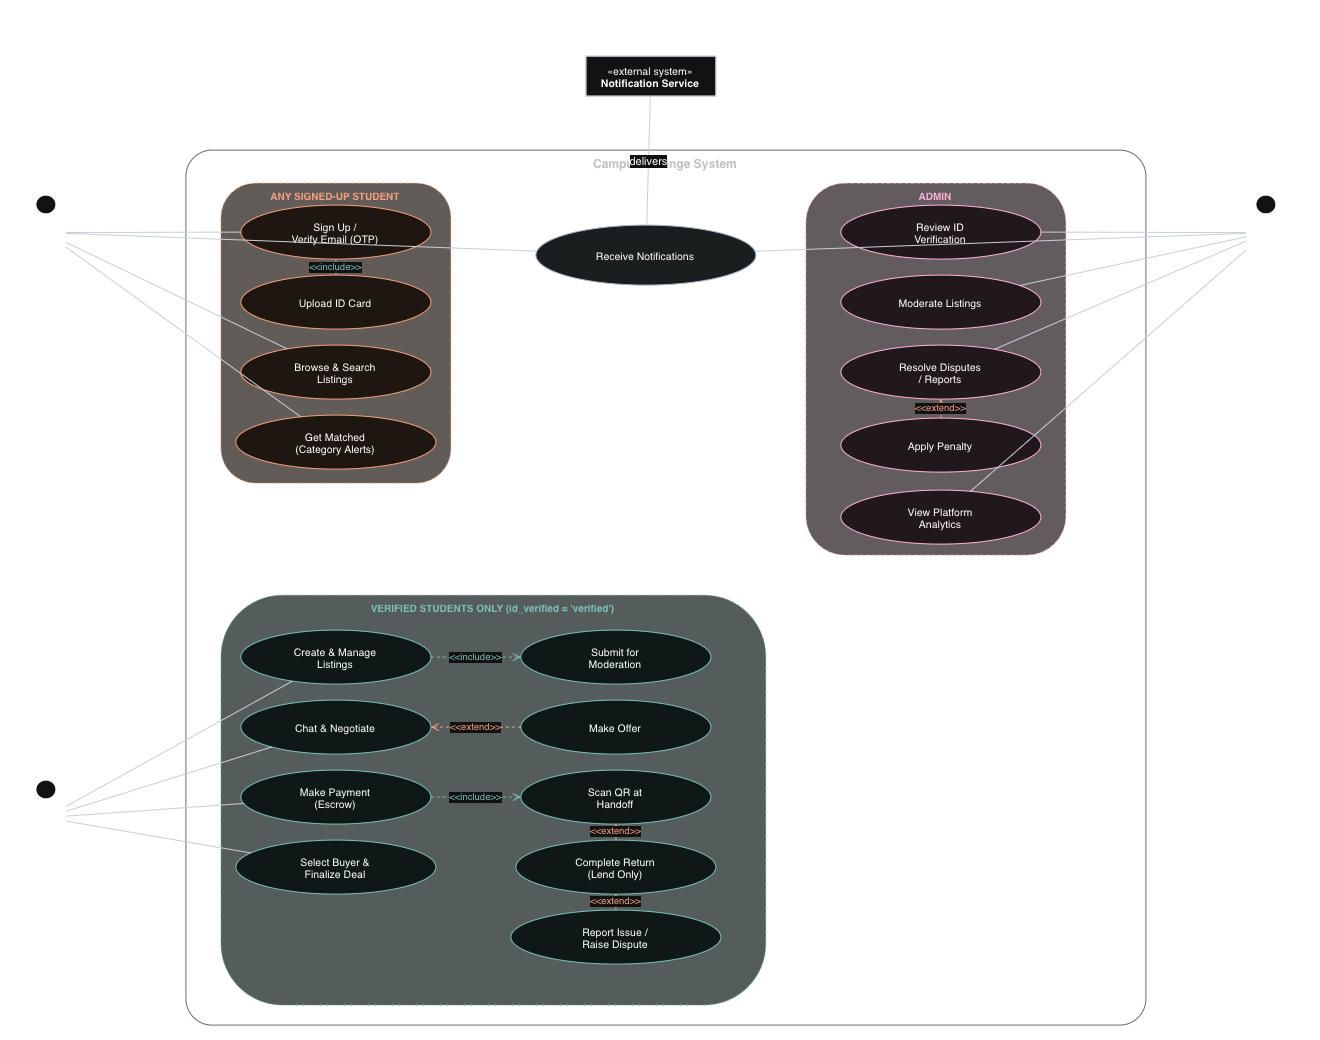
\includegraphics[width=\textwidth]{figures/usecase.png}
  \caption{Use case diagram}
  \label{fig:usecase}
\end{figure}

\section{Class / Entity-Relationship Diagram}
Figure~\ref{fig:er} shows the thirteen database tables with their keys and
constraints.

\begin{figure}[H]
  \centering
  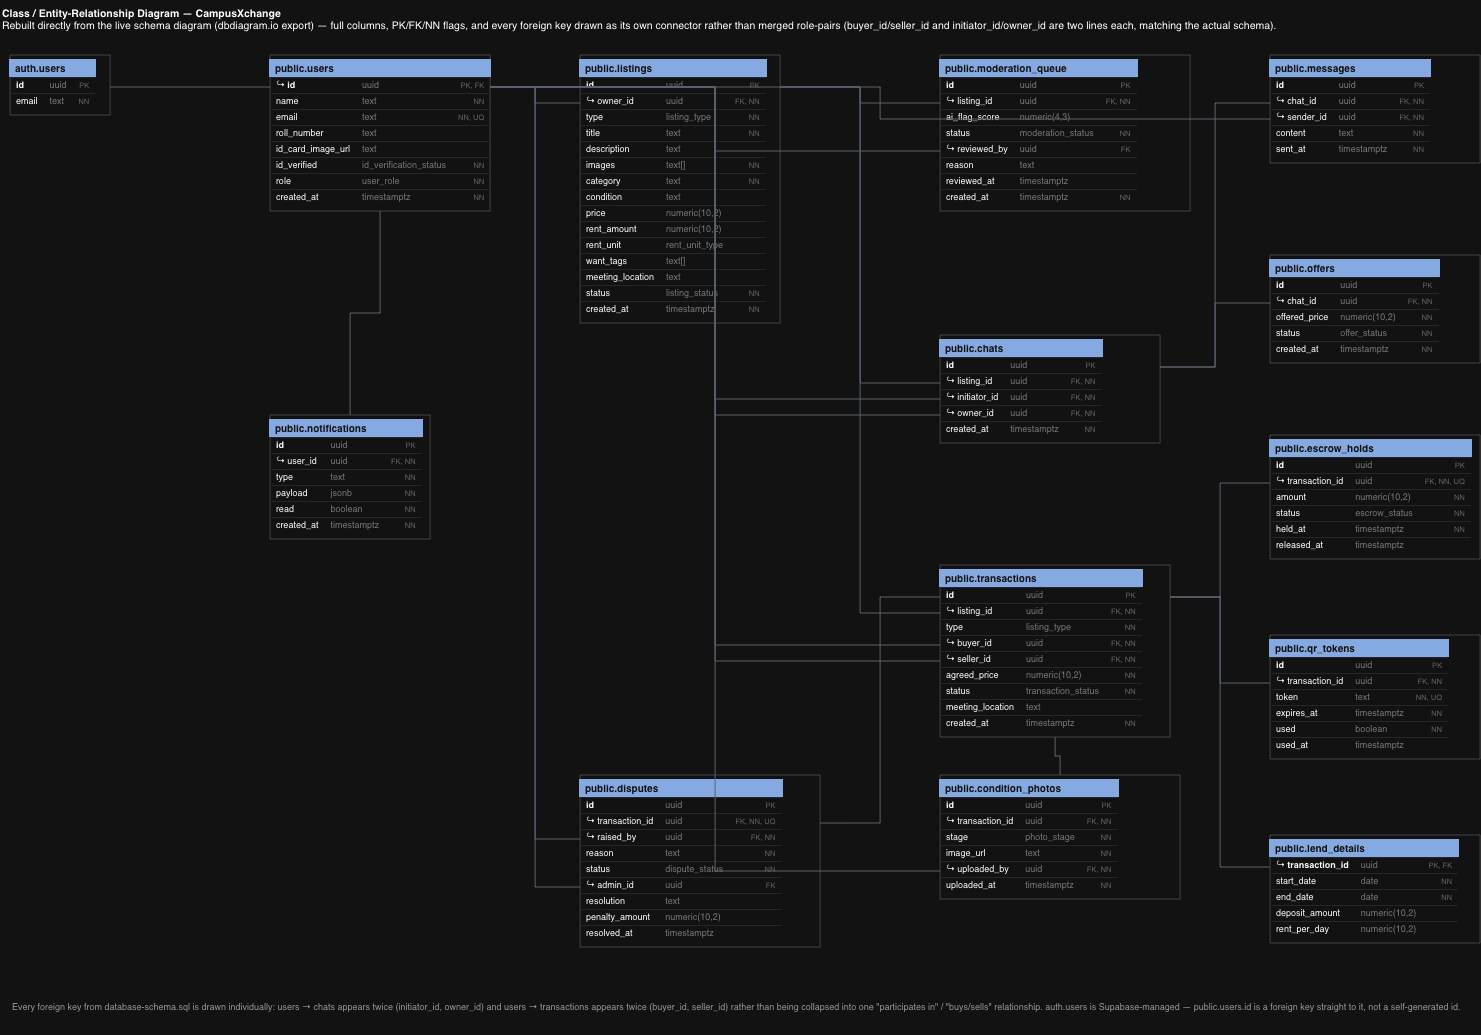
\includegraphics[width=\textwidth]{figures/class-er.png}
  \caption{Class / ER diagram (13 tables)}
  \label{fig:er}
\end{figure}

\section{Data Dictionary}\label{sec:data}
\begin{longtable}{L{3.3cm} L{11.9cm}}
\caption{Database tables}\label{tab:data}\\
\toprule
\textbf{Table} & \textbf{Purpose and key attributes}\\ \midrule\endhead
\texttt{users} & Profile extending Supabase \texttt{auth.users}: id (FK), name, email, roll\_number, id\_card\_image\_url, id\_verified, role, created\_at\\
\texttt{listings} & owner\_id, type, title, description, images[], category, condition, price / rent\_amount + rent\_unit / want\_tags[], meeting\_location, status\\
\texttt{moderation_queue} & listing\_id, ai\_flag\_score, status, reviewed\_by, reason, reviewed\_at\\
\texttt{chats} & listing\_id, initiator\_id, owner\_id; unique (listing\_id, initiator\_id)\\
\texttt{messages} & chat\_id, sender\_id, content, sent\_at\\
\texttt{offers} & chat\_id, sender\_id, offered\_price, status\\
\texttt{transactions} & listing\_id, type, buyer\_id, seller\_id, agreed\_price, status, meeting\_location\\
\texttt{escrow_holds} & transaction\_id (unique), amount, status, held\_at, released\_at\\
\texttt{qr_tokens} & transaction\_id, token (unique), expires\_at, used, used\_at\\
\texttt{lend_details} & transaction\_id (PK), start\_date, end\_date, deposit\_amount, rent\_per\_day\\
\texttt{condition_photos} & transaction\_id, stage (handoff / return), image\_url, uploaded\_by\\
\texttt{disputes} & transaction\_id (unique), raised\_by, reason, status, admin\_id, resolution, penalty\_amount\\
\texttt{notifications} & user\_id, type, payload (JSON), read\\
\bottomrule
\end{longtable}

\section{State Models}
\begin{longtable}{L{3cm} L{12.2cm}}
\caption{Lifecycle states}\label{tab:states}\\
\toprule
\textbf{Entity} & \textbf{States and transitions}\\ \midrule\endhead
Listing & \texttt{pending_review} $\rightarrow$ \texttt{live} (approved) or \texttt{removed} (rejected / deleted); \texttt{live} $\rightarrow$ \texttt{reserved} (buyer selected) $\rightarrow$ \texttt{completed}\\
ID verification & \texttt{pending} $\rightarrow$ \texttt{verified} or \texttt{rejected}; \texttt{rejected} $\rightarrow$ \texttt{pending} on re-upload\\
Offer & \texttt{pending} $\rightarrow$ \texttt{accepted} or \texttt{rejected}\\
Transaction & \texttt{pending_payment} $\rightarrow$ \texttt{escrow_held} $\rightarrow$ \texttt{qr_issued} $\rightarrow$ \texttt{completed}; from \texttt{qr_issued} $\rightarrow$ \texttt{disputed} $\rightarrow$ \texttt{completed} or \texttt{refunded}\\
Escrow & \texttt{held} $\rightarrow$ \texttt{released} or \texttt{refunded}\\
Dispute & \texttt{open} $\rightarrow$ \texttt{under_review} $\rightarrow$ \texttt{resolved}\\
\bottomrule
\end{longtable}

\section{Sequence Diagrams}
\begin{figure}[H]
  \centering
  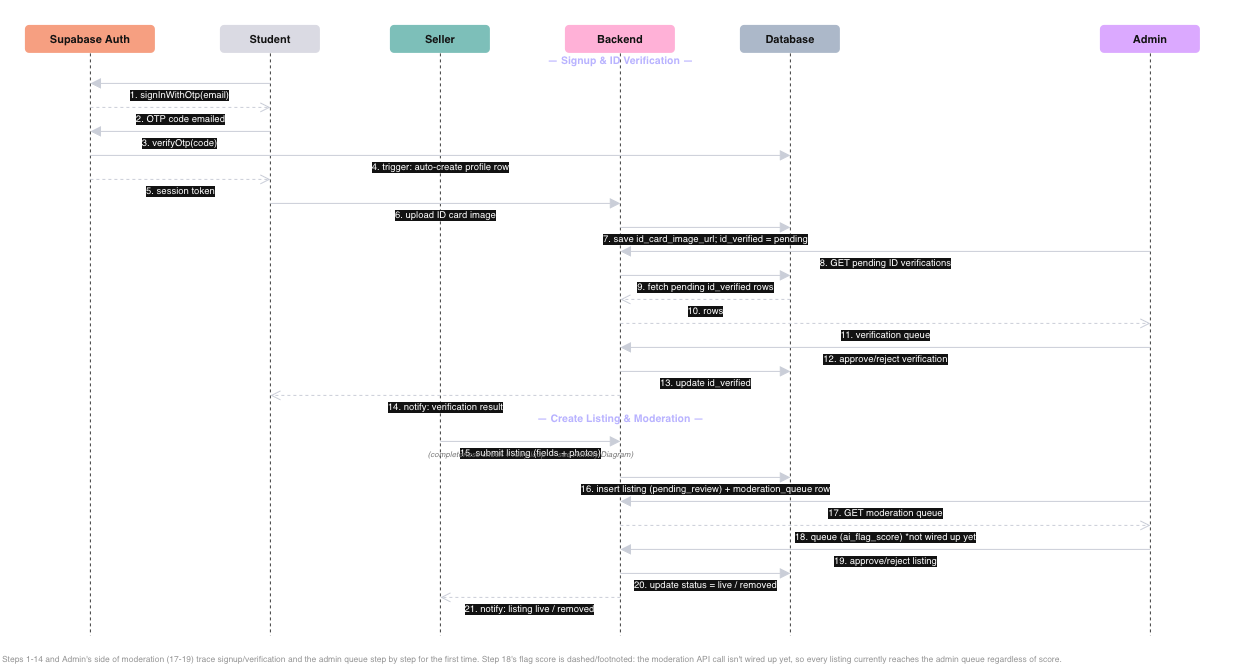
\includegraphics[width=\textwidth]{figures/sequence-1-signup-moderation.png}
  \caption{Sequence diagram 1: sign-up, ID verification, listing and moderation}
\end{figure}
\begin{figure}[H]
  \centering
  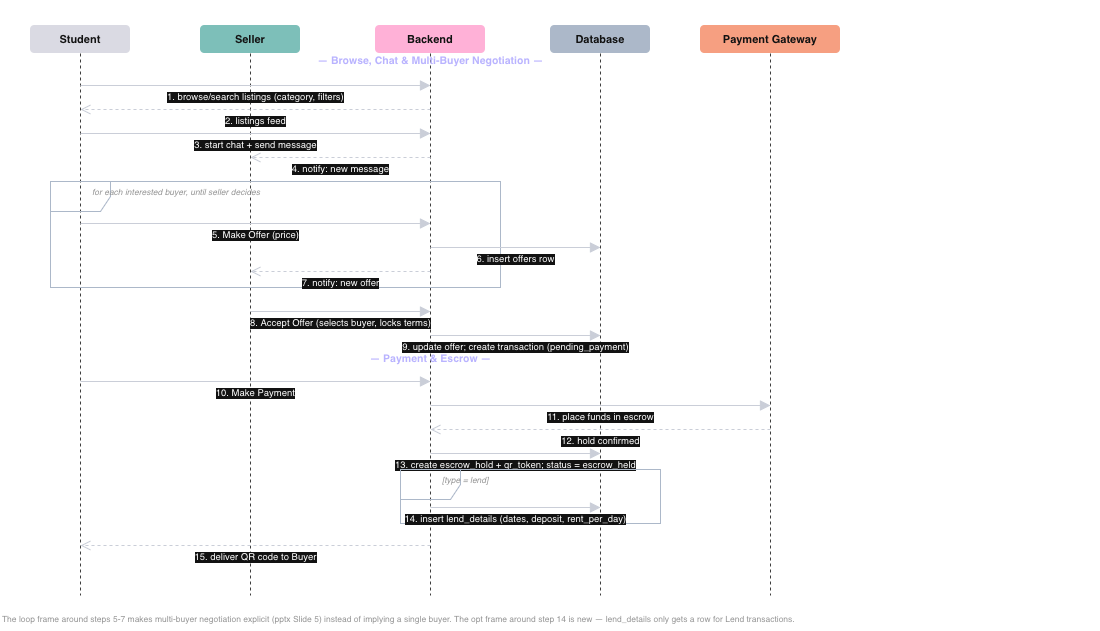
\includegraphics[width=\textwidth]{figures/sequence-2-negotiation-payment.png}
  \caption{Sequence diagram 2: browsing, multi-buyer negotiation, payment and escrow}
\end{figure}
\begin{figure}[H]
  \centering
  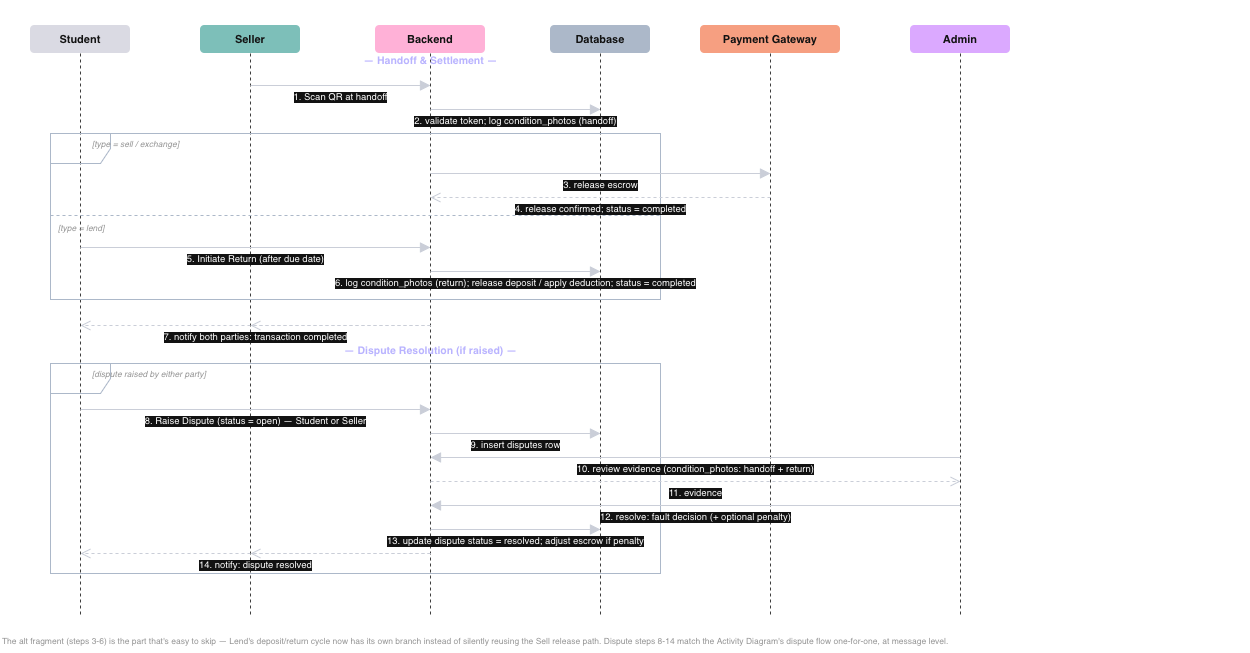
\includegraphics[width=\textwidth]{figures/sequence-3-handoff-disputes.png}
  \caption{Sequence diagram 3: QR handoff, lend return, settlement and disputes}
\end{figure}

\section{Activity Diagrams}
\begin{figure}[H]
  \centering
  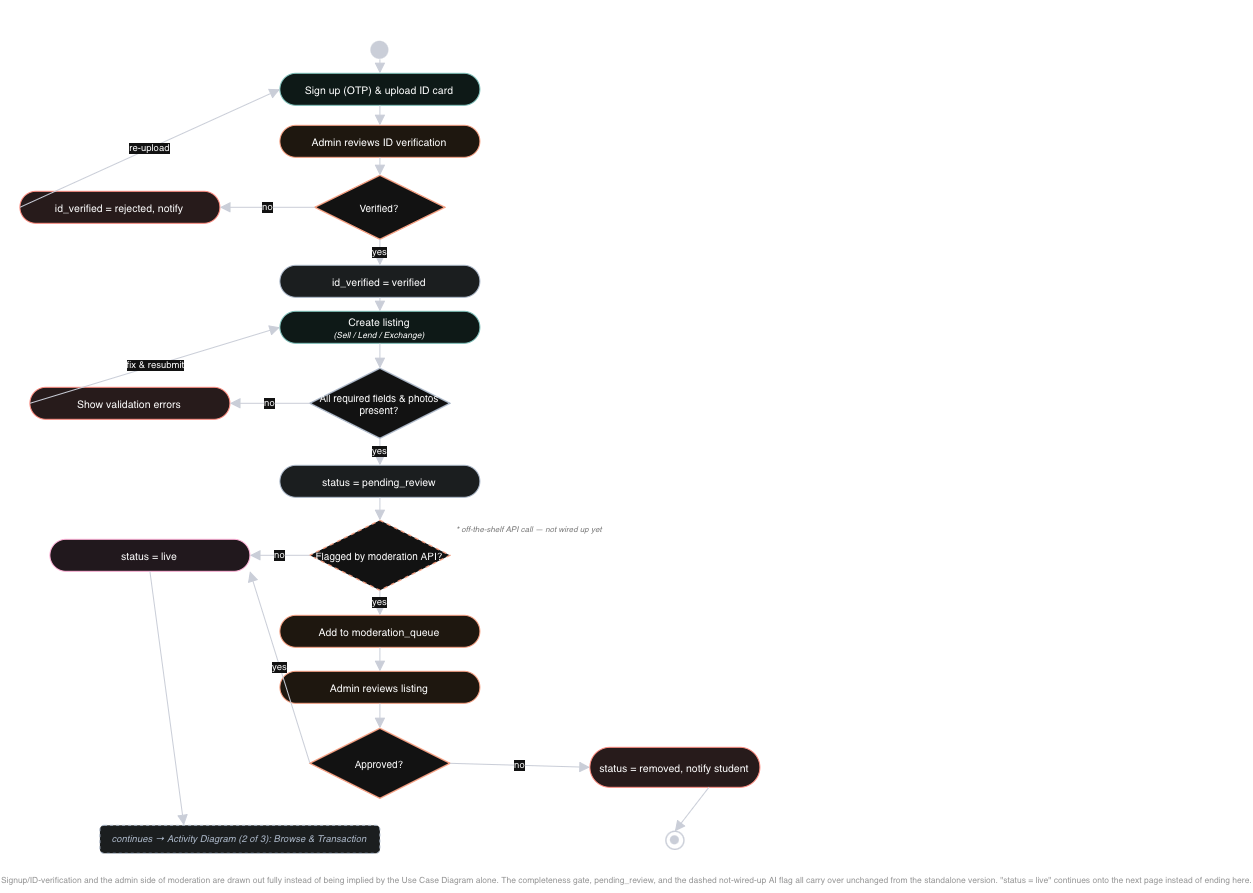
\includegraphics[width=0.85\textwidth]{figures/activity-1-signup-moderation.png}
  \caption{Activity diagram 1: verification and moderation (with rejection loops)}
\end{figure}
\begin{figure}[H]
  \centering
  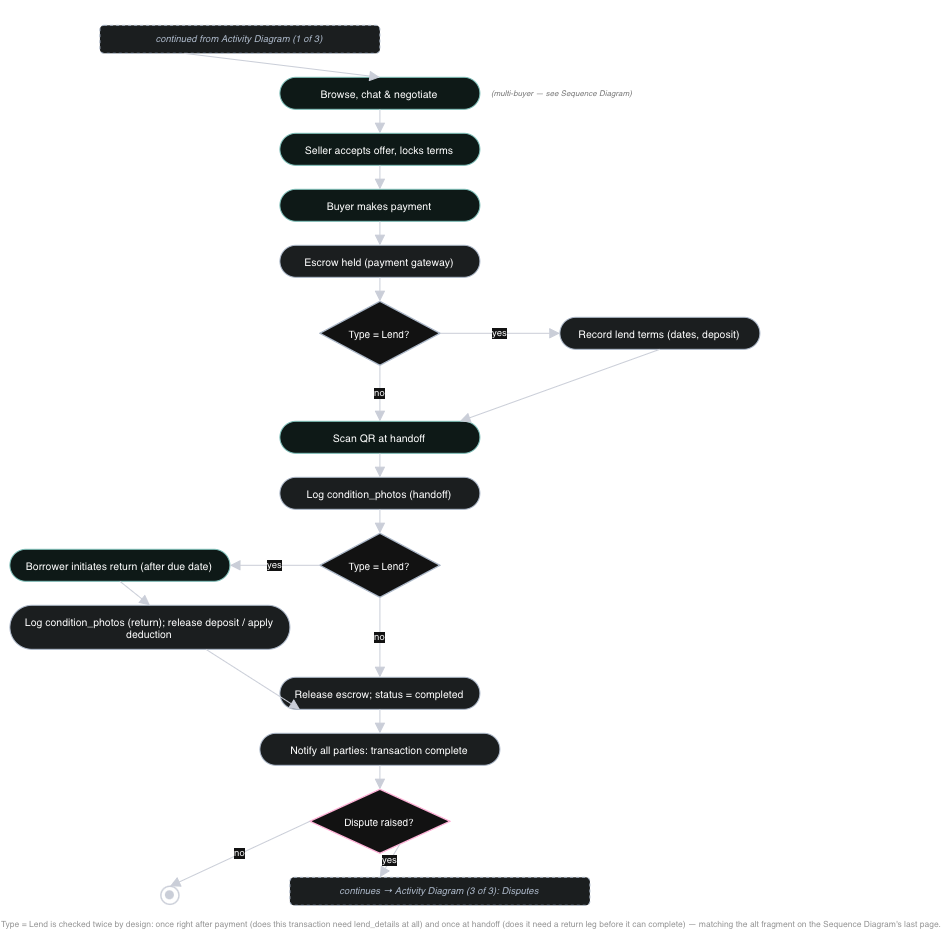
\includegraphics[width=0.72\textwidth]{figures/activity-2-transaction.png}
  \caption{Activity diagram 2: negotiation, payment, handoff and lend return}
\end{figure}
\begin{figure}[H]
  \centering
  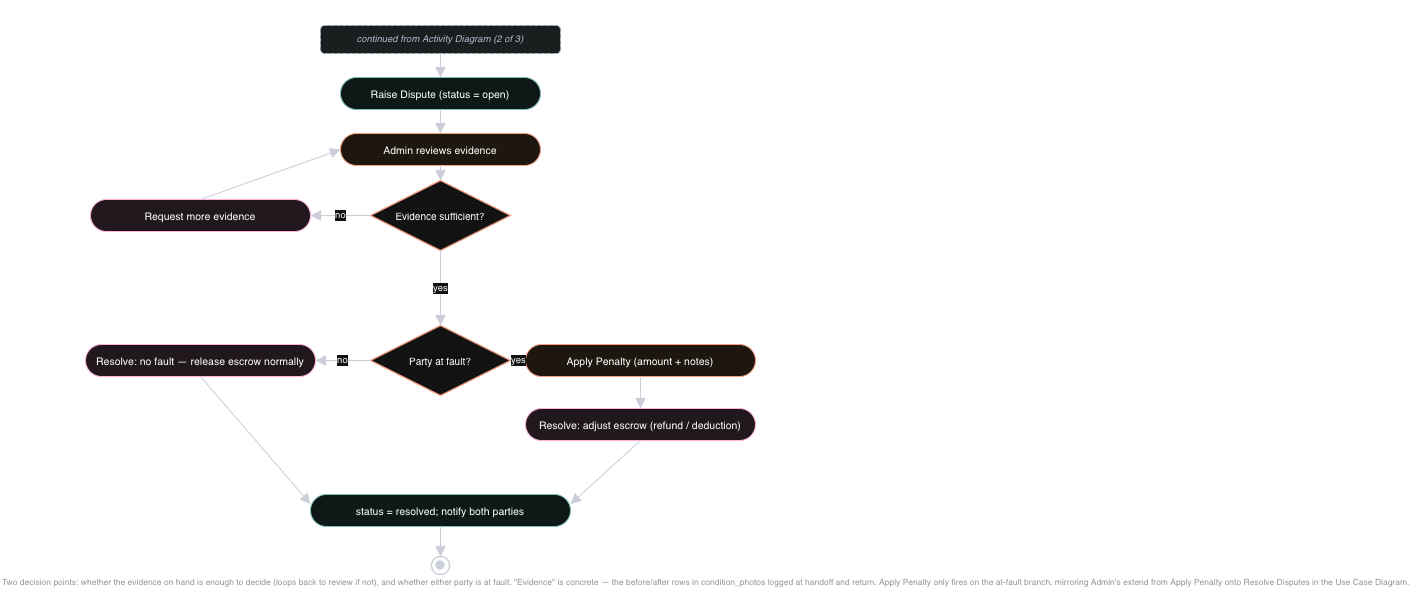
\includegraphics[width=\textwidth]{figures/activity-3-disputes.png}
  \caption{Activity diagram 3: dispute resolution and penalties}
\end{figure}

% =====================================================================
\chapter{Business Rules}
\begin{enumerate}[label=\textbf{BR-\arabic*.}]
  \item Only \texttt{@thapar.edu} email holders may register.
  \item Only verified students may create listings, negotiate, transact or
    raise disputes; guests may only browse.
  \item No listing is visible to others until an administrator approves it.
  \item A user cannot chat on, make offers on, or buy their own listing.
  \item Only the recipient of an offer may accept or reject it; one accepted
    offer closes negotiation in that thread.
  \item The seller chooses which buyer to finalise with when several are
    negotiating.
  \item Money is released to the seller only after a valid QR handoff (and
    return, for lend).
  \item Condition photographs are mandatory at handoff and at return.
  \item Each transaction can have at most one dispute; escrow is frozen
    while it is open.
  \item Automated tools may flag content but never reject, ban or penalise;
    an administrator makes every final decision.
  \item All meetings take place at approved on-campus meeting points.
\end{enumerate}

% =====================================================================
\chapter{Acceptance Criteria and Traceability}

\section{Evaluation Metrics}
\begin{longtable}{L{4.2cm} L{6.6cm} L{3.9cm}}
\caption{Pilot metrics (from the proposal)}\label{tab:metrics}\\
\toprule
\textbf{Metric} & \textbf{Definition} & \textbf{Target}\\ \midrule\endhead
Time to listing clearance (primary) & Submission to moderation decision, from database timestamps & Median $\leq$ 4 hours\\
Transaction completion rate & Agreed transactions reaching QR-verified completion & Tracked; increasing across iterations\\
Lend share and on-time return & Share of lend deals; returns by due date without dispute & Tracked\\
Dispute rate & Lend deals flagged after photo comparison & Tracked; decreasing\\
Off-platform discovery & Pilot users finding/listing in-app vs.\ WhatsApp & Majority in-app\\
User clarity & 1--5 rating of transaction-status clarity & $\geq$ 4\\
Reliability & Uptime of login, listing, payment at peak & $\geq$ 99\%\\
\bottomrule
\end{longtable}
The pilot involves 30--40 students (freshers, graduating seniors and hostel
residents) and 2--3 volunteer moderators.

\section{Traceability Matrix}
\begin{longtable}{L{4.4cm} L{4.4cm} L{5.9cm}}
\caption{Objectives and proposal features traced to requirements}\label{tab:trace}\\
\toprule
\textbf{Objective / pain point} & \textbf{Proposal feature} & \textbf{Requirements}\\ \midrule\endhead
O1 / ``Strangers, no proof'' & Verified access & FR-AUTH-1--10, FR-ADM-3--4, NFR-SEC-1--4\\
O2 / ``No single place to look'' & Sell, Lend, Exchange modules & FR-BRW-1--8, FR-LST-1--9\\
O3 & Trust \& safety layer (moderation) & FR-MOD-1--7, FR-ADM-1--2\\
O4 & In-app chat \& negotiation & FR-CHT-1--10\\
O5 / ``No recourse'' & Payments (escrow), QR handoff & FR-PAY-1--6, FR-HND-1--5\\
O5 / ``Lending has no memory'' & Lend/Borrow module & FR-LND-1--4, FR-PAY-3\\
O6 & Admin dispute handling & FR-DSP-1--6\\
O7 & Evaluation (TLC) & FR-MOD-5, FR-ADM-5\\
\bottomrule
\end{longtable}

% =====================================================================
\appendix
\chapter{Known Gaps and Open Issues}\label{app:gaps}
These are acknowledged differences between this specification and the
current build, to be resolved before the pilot.
\begin{enumerate}
  \item \textbf{Verification gate not enforced on actions.} The backend lets
    any signed-in student create listings and chat; FR-LST-1 and BR-2 require
    \texttt{id_verified = verified}. A guard on these endpoints is needed.
  \item \textbf{Row-Level Security disabled} on all 13 tables (NFR-SEC-5).
  \item \textbf{Chat uses polling} (4 s) instead of WebSockets (FR-CHT-10).
  \item \textbf{Backend not yet deployed}; testing is limited to a shared
    local network (NFR-SCL-2).
  \item \textbf{Payment gateway not yet selected}; the escrow model assumes a
    gateway with hold/release or split-payment support.
  \item \textbf{Penalty tiers} for disputes must be defined before the
    dispute module is built (proposal risk mitigation).
\end{enumerate}

\end{document}
